\begin{frame}
    \frametitle{FHR Benchmark Specifications}
    \begin{itemize}
        \item Several organizations participate in the benchmark with various Monte Carlo
        and Deterministic neutronics software, such as Serpent \cite{leppanen_serpent_2014}, 
        OpenMC \cite{romano_openmc_2013}, and WIMS \cite{lindley_current_2017}. 
        \item UIUC participates in the benchmark with the OpenMC Monte Carlo code 
        \cite{romano_openmc_2013} using the ENDF/B-VII.1 material cross section library 
        \cite{chadwick_endf/b-vii.1_2011}.
        \item The benchmark will have three phases, starting from a single fuel assembly
        simulation without burnup (Phase I), gradually extending to full core depletion
        (Phase II) and multi-physics feedback (Phase III). 
    \end{itemize}
    \begin{table}
        \caption{\acrfull{OECD} \acrfull{NEA} \acrfull{FHR} Benchmark Phases 
        \cite{noauthor_fluoride_nodate}.}
        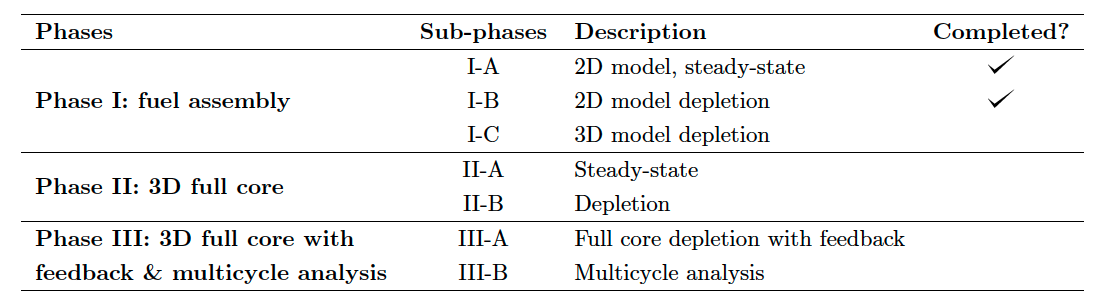
\includegraphics[width=0.8\linewidth]{figures/benchmark-phases.png} 
    \end{table}
\end{frame}

\begin{frame}
    \frametitle{FHR Benchmark Specifications}
    \begin{itemize}
        \item Only Phase I-A and I-B specifications have been released 
        \item Benchmark participants must produce the following results for 
        the 9 cases: $k_{eff}$, reactivity coefficients ($\beta_{eff}$, 
        $\alpha_D$, $\alpha_{T, FliBe}$, $\alpha_M$), fission source distribution, 
        neutron flux distribution, fuel assembly averaged neutron spectrum
    \end{itemize}
    \begin{table}
        \caption{Description of the \acrlong{FHR} benchmark Phase I-A cases 
        \cite{noauthor_fluoride_nodate}.}
        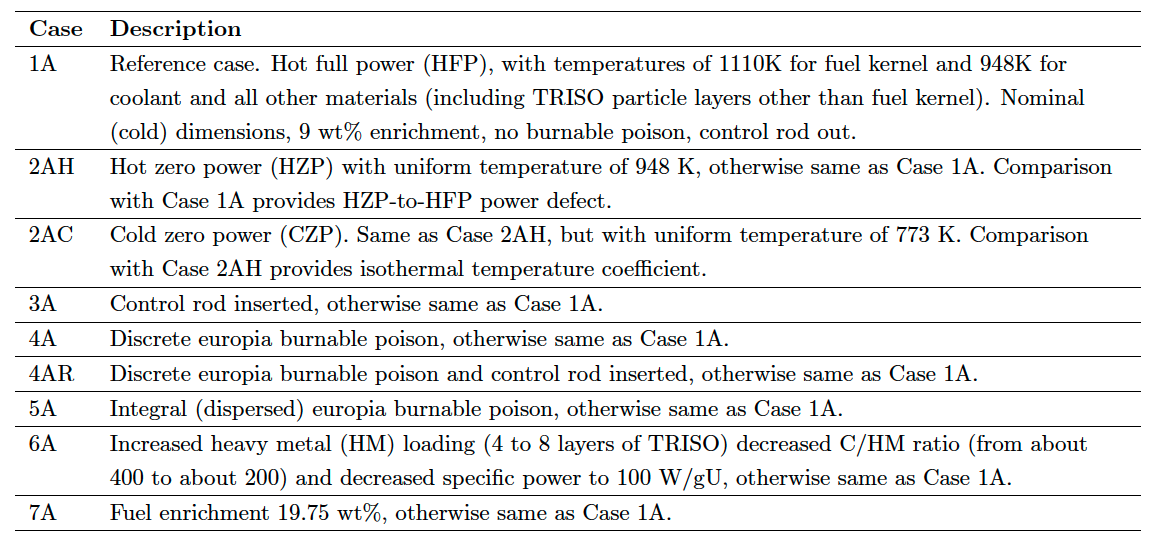
\includegraphics[width=0.8\linewidth]{figures/benchmark-cases.png} 
    \end{table}
\end{frame}